% !TeX encoding = UTF-8
% !TeX spellcheck = en_US
\documentclass{article}
%%%%%%%%%%%%%%%%%%%%%%%%%%%%%%%%%%%%%%%%%%%%%%%%%%%%%%%%%%%%%%%%%%%%%%%%%%%%%%%%%%%%%%%%%%%%%%%%%%%%%%%%%%%%%%%%%%%%%%%%%%%%%%%%%%%%%%%%%%%%%%%%%%%%%%%%%%%%%%%%%%%%%%%%%%%%%%%%%%%%%%%%%%%%%%%%%%%%%%%%%%%%%%%%%%%%%%%%%%%%%%%%%%%%%%%%%%%%%%%%%%%%%%%%%%%%
\usepackage[a4paper,top=2cm]{geometry}
\usepackage{amssymb,amsmath,amsfonts}
\usepackage[english]{babel}
\usepackage[a4paper]{geometry}
\usepackage{enumitem}
\usepackage{booktabs}
\usepackage{csquotes}
\usepackage{graphicx}
\usepackage[numbered,framed]{matlab-prettifier}
\usepackage{url}
%\parindent0mm
%\parskip1.5ex plus0.5ex minus0.5ex
\usepackage[backend=biber,style=authoryear]{biblatex}
\addbibresource{biblio.bib}
\begin{document}
	
\title{Quantitative Macroeconomics}
\author{Midterm Exam}
\date{Winter 2022/2023\\Version 1.0.1}
\maketitle

\section*{General information}
\begin{itemize}
	\item Answer \textbf{all} of the following \textbf{five} exercises in English.
	\item All assignments will be given the same weight in the final grade.
	\item Hand in your solutions before Monday January, 9 2023 at 3pm.
	\item The solution files should contain your executable (and commented) script files
		as well as all additional documentation as \texttt{pdf}, not \texttt{txt}, \texttt{md}, \texttt{tex}, \texttt{doc} or \texttt{docx}.
	Your \texttt{pdf} files may also include scans or pictures of handwritten notes.
	\item Please e-mail ALL the solution files to \url{willi.mutschler@uni-tuebingen.de}.
	I will confirm the receipt of your work also by email (typically within the hour). If not, please resend it to me.
	\item All students must work on their own, please also give your student ID number and the name of the module you want to earn credits for.
	\item It is advised to regularly check Ilias and your emails in case of urgent updates.
	\item If there are any questions, do not hesitate to contact Willi Mutschler.
\end{itemize}

\section*{Changelog}
Version 1.0.1:
\begin{itemize}
	\item Exercise 4: The implied rotated impact matrix should be $\widetilde{B}_0^{-1}=PQ$ and not $\widetilde{B}_0^{-1}=QP$.
\end{itemize}

\newpage

	
\section[Theoretical and Simulated Moments]{Theoretical and Simulated Moments\label{ex:TheoreticalAndSimulatedMoments}}
\begin{enumerate}
 	\item Derive the unconditional first two moments (i.e. theoretical mean, covariance and autocovariance matrix) of the covariance stationary VAR(1) model: $y_t = \nu + A y_{t-1} + u_t$
 	\item Simulate $R=100$ datasets each with $T=100$ observations for
 	\begin{align*}
 	y_t = \begin{pmatrix}0.2 &0.3 \\-0.6 & 1.1 \end{pmatrix} y_{t-1}  + u_t
 	\end{align*}
 	provided that $u_t \sim WN(0,\Sigma_u)$ and $\Sigma_u = \begin{pmatrix}0.9 &  \\ 0.2 & 0.5 \end{pmatrix}$.
	\item Compute the sample mean and sample covariance matrix for each of the $R$ datasets. 
	Then take the average and compare the results with part (1).
	\item How does your choice of $R$ or $T$ change your results?
	
\end{enumerate}

\newpage


\section{Properties Of Lag-Order Selection Criteria}
Assume that the true Data-Generating-Process (DGP) follows the following VAR(4) model
$$y_t = \begin{pmatrix}
2.4 & 1.0\\
0 & 1.1
\end{pmatrix}
y_{t-1}+
\begin{pmatrix}
-2.15 & -0.9\\
0 & -0.41
\end{pmatrix}
y_{t-2}+
\begin{pmatrix}
0.852 & 0.2\\
0& 0.06
\end{pmatrix}
y_{t-3}+
\begin{pmatrix}
-0.126 & 0\\
0 & 0.0003
\end{pmatrix}
y_{t-4}
+ u_t$$
where $u_t$ is a Gaussian white noise with contemporary covariance matrix $\Sigma_u = \begin{pmatrix}
0.9&0.2\\0.2&0.5
\end{pmatrix}$.

Perform a Monte-Carlo analysis to study both the finite-sample as well as asymptotic properties of the Akaike Information Criterion (AIC) and the Schwarz Information Criterion (SIC):
\begin{align*}
AIC(m)  &= \log(det(\tilde{\Sigma}_u(m))) + \frac{2}{T}\varphi(m)\\
SIC(m)  &= \log(det(\tilde{\Sigma}_u(m))) + \frac{\log T}{T}\varphi(m)
\end{align*}
where $\tilde{\Sigma}_u=T^{-1}\sum_{t=1}^T \hat{u}_t\hat{u}_t'$ is the residual covariance matrix estimator for a reduced-form VAR model of order $m$ based on OLS residuals $\hat{u}_t$. The function $\varphi(m)$ corresponds to the total number of regressors in the system of VAR equations. The VAR order is chosen such that the respective criterion is minimized over the possible orders $m = 0,...,p^{max}$. To this end, do the following.

\begin{itemize}
	\item Set the number of Monte Carlo repetitions $R=100$ and $p^{max}=8$.
	\item Initialize output matrices $aic$ and $sic$ each of dimension $R \times 5$. 
	\item For $r=1,...,R$ do the following:
	\begin{itemize}
		\item Simulate $10100$ observations for the DGP given above and discard the first 100 observations as burn-in phase. Save the remaining 10000 observations in a matrix $Y$.
		\item Compute the lag criteria for 5 different sample sizes $T=\{80, 160, 240, 500, 10000\}$, i.e. use the last $T$ observations of your simulated data matrix $Y$ for computations.
		\item Save the chosen lag order in the corresponding output object at position $[r,j]$ where $j=1,...,5$ indicates the corresponding sample size.
	\end{itemize}
	\item Look at the frequency tables of your output objects for the different subsamples. Hint: \texttt{tabulate(aic(:,1))} displays a frequency table for the AIC criterion with sample size equal to 80.
\end{itemize}
Given your results, do you agree with the following (general) findings?
\begin{enumerate}
	\item AIC is not consistent for the true lag order, whereas SIC is consistent.
	\item AIC never (asymptotically) selects a lag order that is lower than the true lag order.
	\item In finite samples, we usually have $\hat{p}_{SIC} \leq \hat{p}_{AIC}$.
	\item In finite samples, AIC has a tendency to overestimate the lag order, SIC has a tendency to underestimate the lag order; hence, one should rely on AIC in finite samples.
\end{enumerate}

\newpage


\section{How Well Does the IS-LM Model Fit Postwar US Data?}
Consider a quarterly model for $y_t = (\Delta gnp_t, \Delta i_t, i_t-\Delta p_t, \Delta m_t - \Delta p_t)'$,
  where $gnp_t$ denotes the log of GNP, $i_t$ the nominal yield on three-month Treasury Bills,
  $\Delta m_t$ the growth in M1 and $\Delta p_t$ the inflation rate in the CPI.
There are four shocks in the system: an aggregate supply (AS), a money supply (MS), a money demand (MD) and an aggregate demand (IS) shock.
Ignoring the lagged dependent variables for \textbf{expository} purposes ($B_1=...=B_p=0$),
  the unrestricted structural VAR model can be simply written as $B_0 y_t = \varepsilon_t$. That is:
\begin{align}
\Delta gnp_t &= -b_{12}\Delta i_t -b_{13}(i_t-\Delta p_t) -b_{14}(\Delta m_t-\Delta p_t) + \varepsilon_t^{AS} \label{eq:AS}\\
\Delta i_t &= -b_{21}\Delta gnp_t -b_{23}(i_t-\Delta p_t) -b_{24}(\Delta m_t-\Delta p_t) + \varepsilon_t^{MS} \label{eq:MS}\\
i_t - \Delta p_t &= -b_{31}\Delta gnp_t -b_{32}\Delta i_t -b_{34}(\Delta m_t-\Delta p_t) + \varepsilon_t^{MD} \label{eq:MD}\\
\Delta m_t - \Delta p_t &= -b_{41}\Delta gnp_t -b_{42}\Delta i_t - b_{43} (i_t-\Delta p_t) + \varepsilon_t^{IS} \label{eq:IS}
\end{align}
where $b_{ij}$ denotes the $ij$th element of $B_0$.
Consider the following identification restrictions:
\begin{itemize}
	\item Money supply shocks do not have contemporaneous effects on output growth, i.e.
	$$\frac{\partial \Delta gnp_t}{\partial \varepsilon_t^{MS}}=0$$	
	\item Money demand shocks do not have contemporaneous effects on output growth, i.e.
	$$\frac{\partial \Delta gnp_t}{\partial \varepsilon_t^{MD}}=0$$	
	\item Monetary authority does not react contemporaneously to changes in the price level.\\Hint: compute
	$$\frac{\partial \Delta i_t}{\partial \Delta p_t}=0$$
	from equation \eqref{eq:MS}.
	\item Money supply shocks, money demand shocks and aggregate demand shocks do not have long-run effects on the log of real GNP:	
	$$\frac{\partial gnp_t}{\partial \varepsilon_t^{MS}}=0,\qquad \frac{\partial gnp_t}{\partial \varepsilon_t^{MD}}=0,\qquad \frac{\partial gnp_t}{\partial \varepsilon_t^{IS}}=0$$	
	\item The structural shocks are uncorrelated with covariance matrix $E(\varepsilon_t \varepsilon_t')=\Sigma_\varepsilon$.
	In other words, the variances are \textbf{not} normalized.
\end{itemize}
Solve the following exercises:
\begin{enumerate}
	\item Derive the implied exclusion restrictions on the matrices $B_0$, $B_0^{-1}$ and $\Theta(1)$.
	\item Consider the data given in the csv file \texttt{gali1992.csv}.
	Estimate a VAR(4) model with constant term.
	\item Estimate the structural impact matrix using a nonlinear equation solver,
	  i.e. the objective is to find the unknown elements of $B_0^{-1}$ and the diagonal elements of $\Sigma_\varepsilon$ such that
	$$\begin{bmatrix}
	vech(B_0^{-1} \Sigma_\varepsilon B_0^{-1'}-\hat{\Sigma}_u)\\
	\text{short-run restrictions on }B_0 \text{ and } B_0^{-1} \\
	\text{long-run restrictions on }\Theta(1)\\
	\end{bmatrix}$$
	is minimized.
	Normalize the shocks such that the diagonal elements of $B_0^{-1}$ are positive.
	\item Use the implied estimates of $B_0^{-1}$ and $\Sigma_\varepsilon$ to plot the structural impulse responses functions
	for (i) real GNP, (ii) the yield on Treasury Bills, (iii) the real interest rate and (iv) real money growth.
\end{enumerate}

\newpage

\section[Sign-identified Monetary SVAR Model for US]{Sign-identified Monetary SVAR Model for US\label{ex:SignIdentifiedMonetarySVARUS}}
Consider data for $y_t = (\Delta gnp_t,\Delta p_t,i_t)'$,
  where $gnp_t$ denotes the log of U.S. real GNP,
  $p_t$ the consumer price index in logs,
  and $i_t$ the federal funds rate.
  Data is given in the csv file \texttt{MonPol.csv} containing the sample period of 1970Q1 to 2011Q1.

We will use the following sign restrictions pattern to identify the structural shocks:
\begin{align}
B_0^{-1}=\begin{bmatrix}
	+ & + & -\\
	+ & - & -\\
	+ & *  & +
	\label{eq:signpattern}
\end{bmatrix}
\end{align}
where $*$ denotes an unrestricted value.

\begin{enumerate}
\item Read the short summary paper by \textcite{Wolf_2022_WhatCanWe} and provide economic intuition for the pattern given in equation \eqref{eq:signpattern}.
\item Write a script that estimates the structural impulse response function via sign restrictions.
To this end:
	\begin{itemize}
	\item Estimate a VAR(4) model with constant by using ordinary least-squares.
	Compute the lower Cholesky decomposition of your estimated residual covariance matrix, i.e. $P=chol(\hat{\Sigma}_u)$.
	\item Set the IRF horizon $H=20$ and the number of required sign-identified draws to $N=1000$.
	\item Initialize an array \texttt{IRFvals} of dimension
	(i) number of variables $K$ by (ii) number of shocks $K$ by (iii) horizon $H$ by (iv) number of draws $N$.
	This array will store $n=1,...,N$ sign-identified impulse response functions $\theta_{jkhn}$ for variable $j=1,...,K$
	with respect to shock $k=1,...,K$ at horizon $h=0,...,H$, where $K$ is the number of variables.
	
	\item Initialize \texttt{n=1} and write a while loop that executes the following steps:
		\begin{itemize}
		\item Draw an orthogonal rotation matrix $Q$ using the function \texttt{drawRotationMatrixQ.m} in the appendix.
		\item Compute the implied rotated impact matrix $\widetilde{B}_0^{-1}=PQ$.
		\item Note that $\widetilde{B}_0^{-1}$ is a valid impact matrix, because $\hat{\Sigma}_u = \widetilde{B}_0^{-1} \widetilde{B}_0^{-1'}$.
		However, we will only accept those impact matrices $\widetilde{B}_0^{-1}$ that fullfill the sign restrictions in equation \eqref{eq:signpattern}.
		Therefore, use if statements to check whether $\widetilde{B}_0^{-1}$ is a valid impact matrix:
		\begin{itemize}
			\item If the pattern is correct, increase $n$ by 1 and compute the implied IRFs. Store these into \texttt{IRFvals(:,:,:,n)}.
			\item If the pattern is incorrect, don't change the value of $n$, discard this draw and go back to the beginning of the loop.
			\end{itemize}
		\item End the while loop if \texttt{n=N}.
		\end{itemize}
	\item Plot \textbf{ALL} $N$ impulse response functions that fullfill the sign pattern for (i) the level of GDP, (ii) CPI inflation and (iii) the Federal Funds rate.
	\\Hint: The graphs should look similar to figure \ref{fig:signSVAR} in the appendix.
	That is, in each subplot compute and plot \texttt{IRFS = squeeze(IRFvals(ivar,ishock,1:nsteps,:))}.	
	\end{itemize}
\end{enumerate}


\newpage

\section[ChatGPT and Sign-identified SVAR Models]{ChatGPT and Sign-identified SVAR Models\label{ex:ChatGPTSignSVAR}}
From the media you've probably heard much buzz about ChatGPT,
  which is a natural language processing tool driven by fancy AI technology.
Particularly, it is supposed to be able to answer all of your exam questions.
So, consider the following output of ChatGPT:
\\~\\
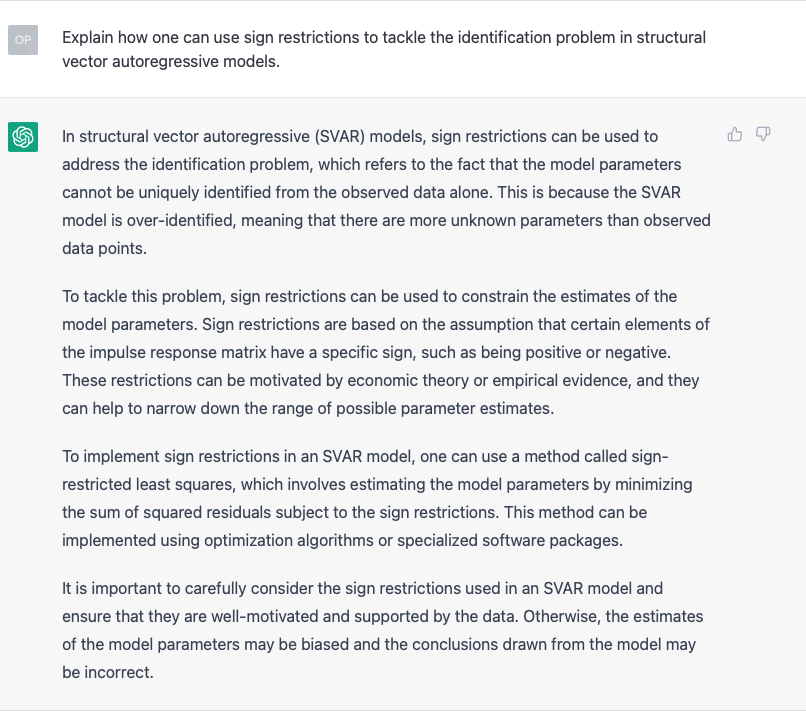
\includegraphics[width=\textwidth]{plots/ChatGPTSignRestrictions.png}
~\\
\noindent Read the short summary paper by \textcite{Wolf_2022_WhatCanWe} (or the exhaustive chapter in \textcite[Ch.~13]{Kilian.Lutkepohl_2017_StructuralVectorAutoregressive})
on sign-identified SVAR models and comment on the accuracy of the answer ChatGPT gave.
Particularly, point out the parts that are incorrect.


\newpage


\appendix

\printbibliography
\newpage
\section{Codes}
\lstinputlisting[label=drawRotationMatrixQ,title=\lstname,style=Matlab-editor,basicstyle=\footnotesize\mlttfamily]{progs/matlab/drawRotationMatrixQ.m}

\newpage

\section{Figures}
\begin{figure}[htbp]\caption[]{Sign-identified IRFs}\label{fig:signSVAR}
	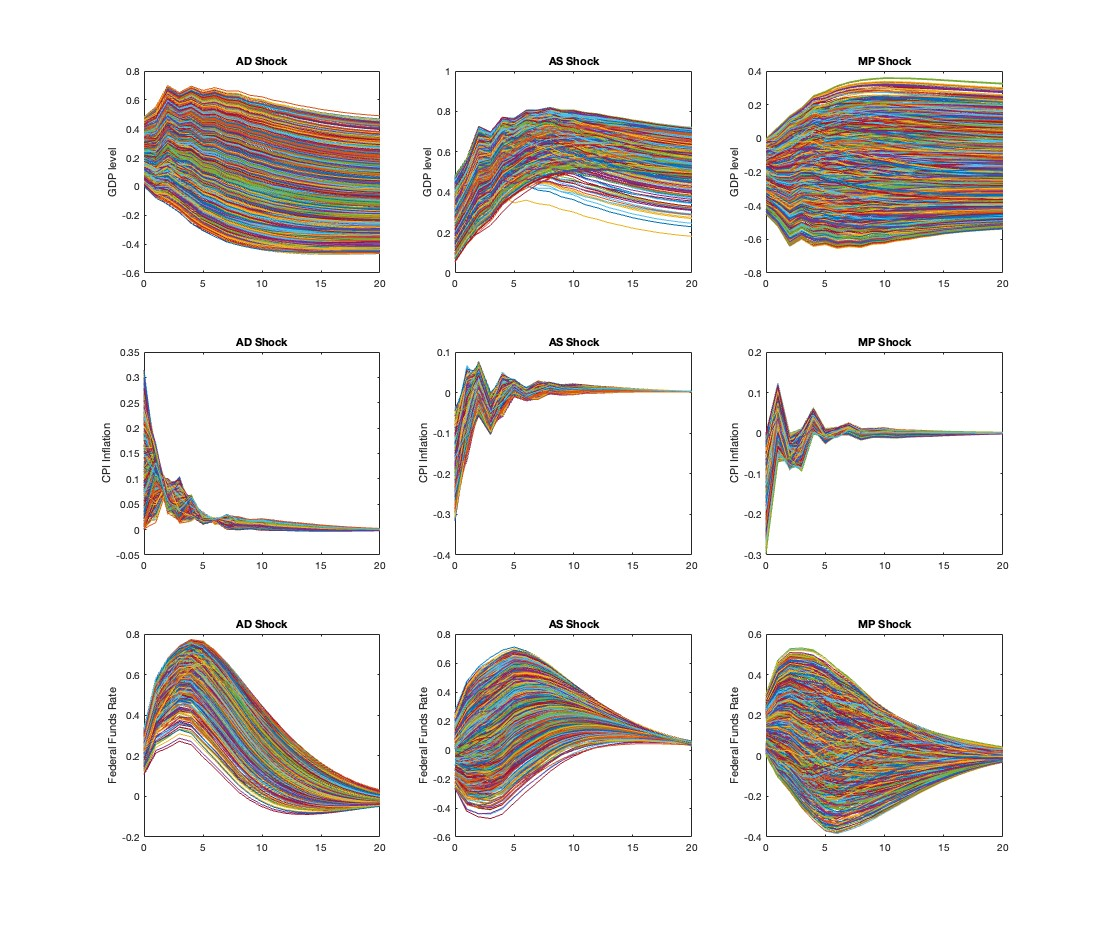
\includegraphics[width=\textwidth]{plots/signIRFs.jpg}
\end{figure}

\end{document}
